
\documentclass[12pt]{article}
\usepackage[english]{babel}
\usepackage[utf8x]{inputenc}
\usepackage{amsmath}
\usepackage{graphicx}
\usepackage{hyperref}
\usepackage{float}
\usepackage[colorinlistoftodos]{todonotes}
\usepackage{biblatex}
\usepackage{setspace}
\usepackage{geometry}
\geometry{left = 1in}
\geometry{right = 1in}
\geometry{top = 1 in}
\geometry{bottom = 1 in}
\addbibresource{bib.bib}

\begin{document}

\noindent Project Report in Partial Fulfillment of Spring 2021 EC/ME/SE 543 Course Requirements\\ \\Title: Analysis of February 2021 Texas Power Outage, Power Market and How to Move Forward\\ \\Date Submitted: May 03, 2021\\ \\ Acknowledgement: \\ \\ As the sole author of this report I certify that I am aware of the following citation/referencing requirements and that failure to abide by them may result in academic misconduct disciplinary action and a failing grade.
\begin{itemize}
    \item All passages, figures, tables, graphs and any other material lifted from a web site document, an existing report whether archived or informally made available to me, must be included in quotes and referenced in the text by exact bibliographic form and page number.
    \item The above holds for paraphrased or modified information or ideas taken from any source. In this case the reference should appear at the bottom of a table or graph or end of a paragraph without quotes.
\end{itemize}\\ \\ Furthermore, I certify that I have carefully followed the above requirements in putting together the
paper that follows.\\ \\ Name: Christopher Lemus \\ \\ Signature: \\ 
\includegraphics[scale = 0.3]{signature.png}

\clearpage
\begin{titlepage}

\newcommand{\HRule}{\rule{\linewidth}{0.5mm}} % Defines a new command for the horizontal lines, change thickness here

\center % Center everything on the page

\textsc{\LARGE Boston University}\\[1cm] % Name of your university/college

\includegraphics[scale=0.1]{2000px-boston_university_wordmark.jpeg}\\[1cm] % Include a department/university logo - this will require the graphicx package
\textsc{\Large Sustainable Power Systems: Planning, Operation and Markets}\\[0.5cm] % Major heading such as course name
\textsc{\large ENG EC 543}\\[0.5cm] % Minor heading such as course title

\HRule \\[0.4cm]
{ \huge \bfseries Analysis of February 2021 Texas Power Outage, Power Market and How to Move Forward}\\[0.4cm] % Title of your document
\HRule \\[1 cm]

\begin{minipage}{0.4\textwidth}
\begin{flushleft} \large
\emph{Author:}\\
Christopher \textsc{Lemus\footnote{E-Mail: lemusc@bu.edu}}\\ % Your name
\end{flushleft}

\affil{Department of Electrical Engineering, Boston University}

\end{minipage}\\[1.5cm]



%\vfill % Fill the rest of the page with whitespace

\end{titlepage}
\doublespacing
\newpage
\tableofcontents
\newpage

\section{Introduction}
\indent %Add more to intro? 
\indent In the month of February 2021, Texas was subject to some of the worst winter storms that it has seen in the last decade. As a result from these storms, massive power outages across the entire state took place due to high demand and the inability to meet demand. Needless to say, the Texas power grid was poorly equipped to endure the freezing temperatures and led to series of distribution errors from within the power grid. The state of Texas should have learned from this mistake a decade ago and should have made drastic progressive steps towards a modern power grid when a very similar situation occurred in February 2011 \cite{TexasMonthly}. The overseeing organization of the Texan power grid, Electric Reliability Council of Texas, or ERCOT, should have been more proactive in protecting their power grid, not just to prevent a catastrophe like this from happening in the future, but to save the lives of the residents of the state of Texas and tens of billions of dollars in damages which could have been invested into the power grid. \par
\indent In this report there will be a thorough discussion on the events that led up to the catastrophic power outages across Texas in February, the reasoning behind the actions that ERCOT has been making in the electric market, errors that have been made and how making the effort to invest into the Texan network while considering new technologies and strategies will save billions of dollars in the long run of damages and repairs from catastrophic outages. Proposals for technologies which could prevent these events in the future will also be discussed. The main purpose this paper will serve to not deter ERCOT but propose more ideal circumstances which would benefit the state of Texas, its power grid, ERCOTs electric market and Texas' residents. \par 
\clearpage
\section{The Texan Power Grid}
\indent%This section will be covering the Texan Power grid, its limitations, its pricing in the market to its customers, why its appealing to the consumers, how well it meets demand, federal regulations by FERC, and technology which makes it predated. 
\indent Texas is the only state in the U.S. which has its own power grid. The reason why ERCOT has not merged with neighboring grids is because they do not want to deal with federal organisations like the Federal Energy Regulatory Commission, or FERC \cite{texTribune}. In addition, ERCOT has not merged with neighboring grids to keep the electricity market price low as shown in the price duration curve in Figure 9, where zonal prices are shown for every hour in the year (8,760 hours per year) and the number of hours in which prices will be higher than the mean of \$30. ERCOT must follow rules which FERC sets which mainly requires them to guarantee demand. The way ERCOT operates their electricity market is entirely up to them and not regulated by the FERC. ERCOT also does not trade significant amounts of power across state lines which further disqualifies ERCOT from needing to abide by FERC regulations \cite{UtilDive}. Another driving factor for Texas overseeing its own power grid is due to them being the number one natural gas and crude oil producing state in the U.S. in which natural gas accounted for 26\% and crude oil accounted for 43\%  in the entire U.S.\cite{TexEnergyProf}. This means that Texas can drive its own power plants and generators to meet the state's demands without needing to depend on other entities and buying energy sources at higher prices for the electricity market. In the year 2020, Texas' number one energy source came from natural gas at approximately 45.5\% as shown in Figure 1 \cite{ERCOTfactSheet}. ERCOT supplies about 85\% of electrical demand to Texas while the other 15\% is covered by either the western interconnection or eastern interconnection and their respective councils (WECC, SERC and SPP) \cite{SGiT}. \par 

\begin{figure}[h!]
\centering
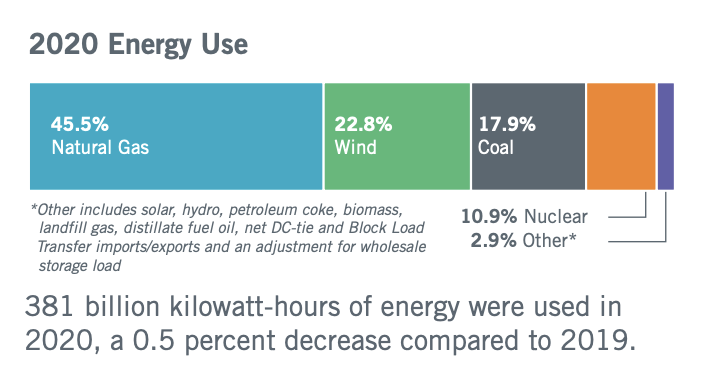
\includegraphics[width=0.65\textwidth]{ERCOT 2020.png}
\caption{\href{http://www.ercot.com/content/wcm/lists/219736/ERCOT_Fact_Sheet_4.22.21.pdf}{ERCOT 2020 Energy Use Sources}}
\end{figure}

\indent %write about Energy only market & no capacity market, coperation of LMP market, incorporation ORDC which translates to price aadder% 
Another caveat of the the Texan market is that it operates as an energy only market with no capacity market \cite{UtilDive}. Capacity markets are aiming to ensure grid reliability by paying participants to guarantee generation for a specified number of years, while energy markets pay their generators on a day-to-day basis for what they provide \cite{UtilDiveMarkets}. Advantages of the energy market in terms of distribution of energy are that there exists capacity reserves, which are a percentage of generated energy that are stored as reserves \cite{EOM}. These reserves are minimal and are mainly used for frequency management when there is too much power generated and flowing through the transmission network or too much demand that can't be met. From these reserves ERCOT is able to trigger the emergency response service (ERS) which allows certain generators and reserves to kick in power where needed to stabilize the frequency \cite{ERS}. The ERS plays a big roll in preventing load shedding, or rolling blackouts, which are meant to distribute power across a network to prevent too much load at a single source. Load shedding was critical in the case of the Texas outage in February 2021 because it helped keep the power grid as stable as possible under the severe stress it was under while rotating power to certain neighborhoods in Texas which needed power so that more residents did not last longer than they needed to in the sub-freezing temperatures. However, the efficiency of the rotating blackouts could have been better and optimized if parts of the grid were modernized (more on this later in the report). \par 
\indent The Texan power grid also operates as a locational market pricing (LMP) market which describes the price at which independent system operators (ISO) can buy and sell electricity in the electricity market. These ISOs will operate using the Day Ahead Market (DAM) and the Real Time Market (RTM) to fund the predicted power needed for the following day and any additional demand that needs to be met which was not met from the DAM through the RTM \cite{LMPdeff}. RTM prices are much more volatile because of the sudden need for generators to generate and meet demand, which ramps up prices and may lead to scarcity pricing like during the outage in February 2021 \cite{ScarcityPricing}. ERCOT also operates under consideration of the Operating Demand Reserve Curve (ORDC) which reflects a higher Price of Reserves for tighter Available Reserves as seen in Figure 2 \cite{ScarcityPricing}. Some implications of the ORDC are that it will maintain the price of energy at a favorable range for those consumers while available reserves are around 4,000 MWs and greater. Once available reserves star going scarce the price of reserves start going scarce; when available reserves reach 2,000 MWs the price of reserves goes to the VOLL price cap. The determination of the ORDC comes from the Loss of Load Probability (LOLP), which gives the probability at which a disturbance or event requires more power than what the real-time reserves have to offer \cite{ORDCLOLP}. If such an event occurs then there will be a drop in frequency in the system transmission network which will call for an energy emergency alert (EEA) and load shed to stabilize the frequency. The ORDC applies a value of lost load (VOLL) of $\frac{\$9,000}{MWh}$ of when available reserves are 2,000 MWh and below. This is because when there are nearly no more reserves available companies need to start paying in the real-time market to generate electricity to meet the demand. All of these factors played enormous roles during the outage as we will see in the following section. 

\begin{figure}[h!]
\centering
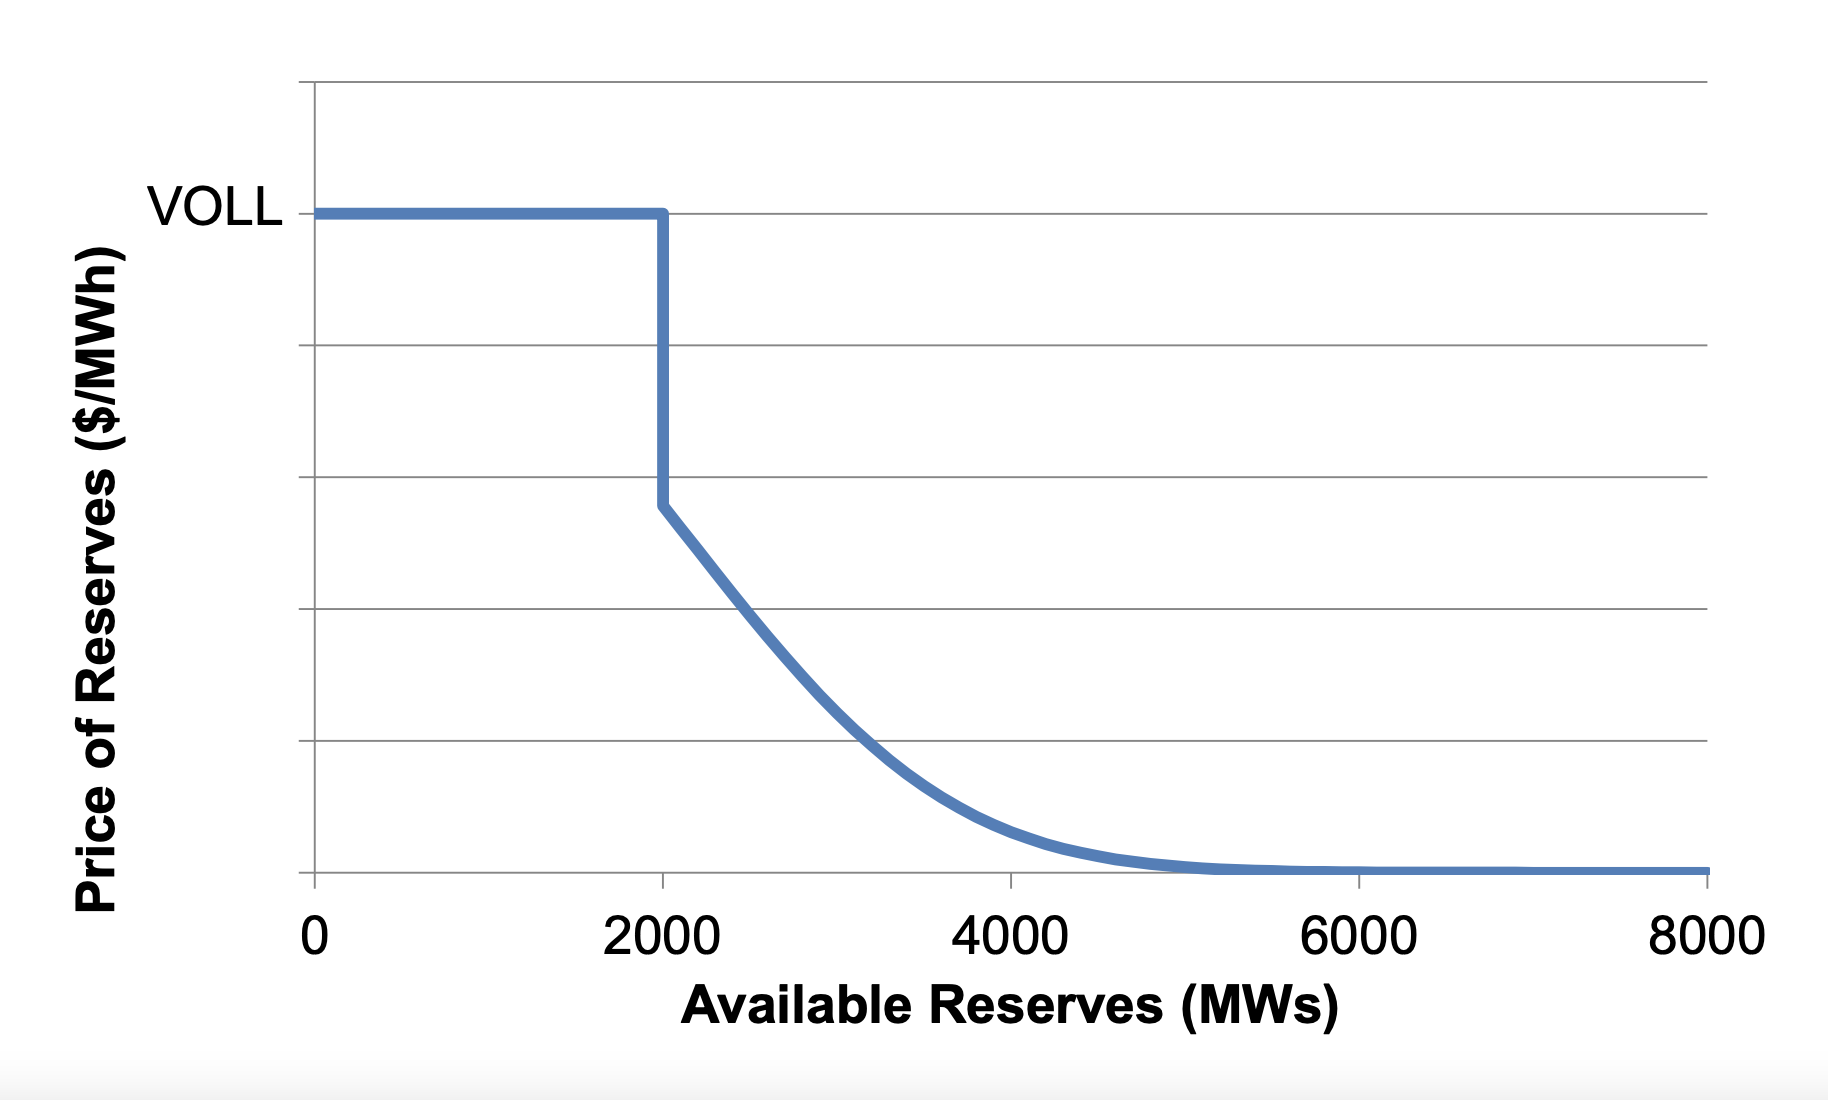
\includegraphics[width=0.45\textwidth]{ORDC Curve.png}
\caption{\href{http://www.ercot.com/content/wcm/training_courses/107/ordc_workshop.pdf}{ERCOT ORDC Curve Model}}
\end{figure}

\newpage
\section{Causes of the February 2021 Blackouts}
\indent %discuss events, and higher demand + low generation causing scarcity pricing cite{scarcityPricing}
\indent The timeline and full summary of the power outages in February 2021 can be found on the site Power Technology Research in an article written by Kamil Maqsood cited here \cite{FreqGraph}. The events will be quickly summarized in the following paragraph.\par
\indent ERCOT and the Texas forecasters were aware of the cold air jet stream that was about to come down across Texas on the weekend of February 13, 2021. There were many alerts and headlines in the news about the freezing temperatures that Texas was going to encounter, but the residents were not prepared for what became multi-day power outages across the state of Texas. On the night of the the 13 of February the temperatures in Texas were beginning to go freezing (32$^{\circ}$F and below) with Houston even going subzero at one point \cite{HoustFreeze}. Due to the sudden freeze and immense cold the residents of Texas became heavily reliant on electricity to heat their homes. The temperature drop caused a surge in demand that was unexpected and in little time the few reserves which Texas had were at maximum capacity and ERCOT had to rely on the Operating Reserve Demand Curve (ORDC) to set scarcity prices for the reserves left over as shown in Figure 2. This surge in demand can also be seen in Figures 3 and 4 which show the Day Ahead Prices and Real-time Prices of the period in which the power outages occurred. It is clear that the the DAM and RTM were maxed out in the limit set by the ORDC - which is $\frac{\$9,000}{MWh}$ - for a handful of days because generation was struggling to meet demand. The reason for generation not being able to keep up with demand were due to distribution reasons, like frozen pipelines and thus discontinuities in the network which are supposed to provide natural gas which is used for power generation at the sites. As a consequence of ERCOTs main energy sources not being able to meet the demand there was a drop in frequency of the electricity generated and in the span of minutes the frequency dropped below the threshold frequency for 4 minutes as can be seen in Figure 5. If the frequency were to have remained below 59.4 Hz for any longer there would have been more generators that would have tripped and caused further blackouts across the state of Texas, leading to more damages to the network, resident property and losses of life. \par
\indent The inability to efficiently rotate blackouts was a big problem because this is what was causing the most harm to families and households. According to an article written by Andrew Engblom, Justin Horwath and Mark Watson and statistics used from NERC, at one point there was a 20 Gigawatt load shed ordered by ERCOT in order to maintain stability in the power grid \cite{loadshed}. These load shed orders caused a cascade effect of problems: no electricity, no food and no water. The load shed events also caused millions of dollars of lost money as well, especially at the VOLL price cap set by ORDC. 

\begin{figure}[h!]
\centering
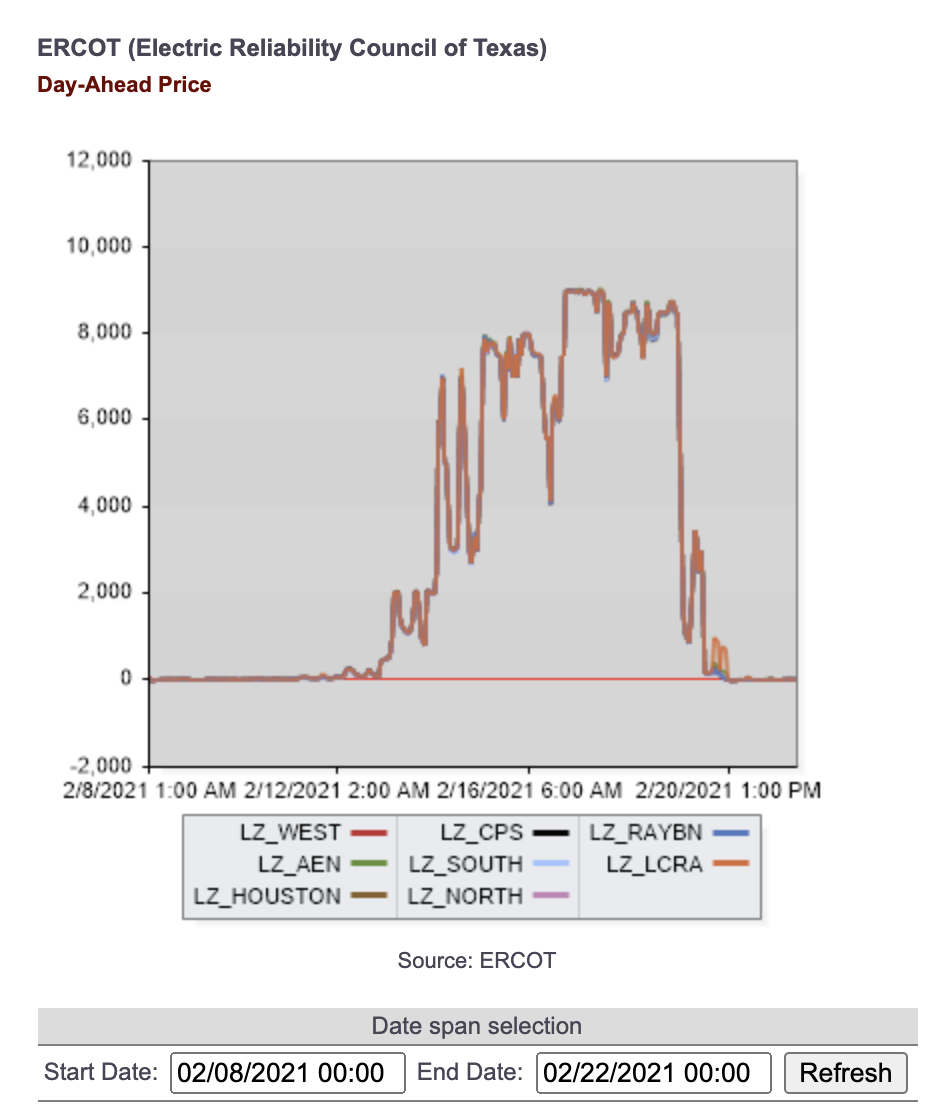
\includegraphics[width=0.65\textwidth]{DAM.png}
\caption{\href{http://www.energyonline.com/Data/GenericData.aspx?DataId=23&ERCOT___Day-Ahead_Price}{ERCOT Day Ahead Prices from Feb. 08, 2021 - Feb. 22, 2021}}
\end{figure}

\begin{figure}[h!]
\centering
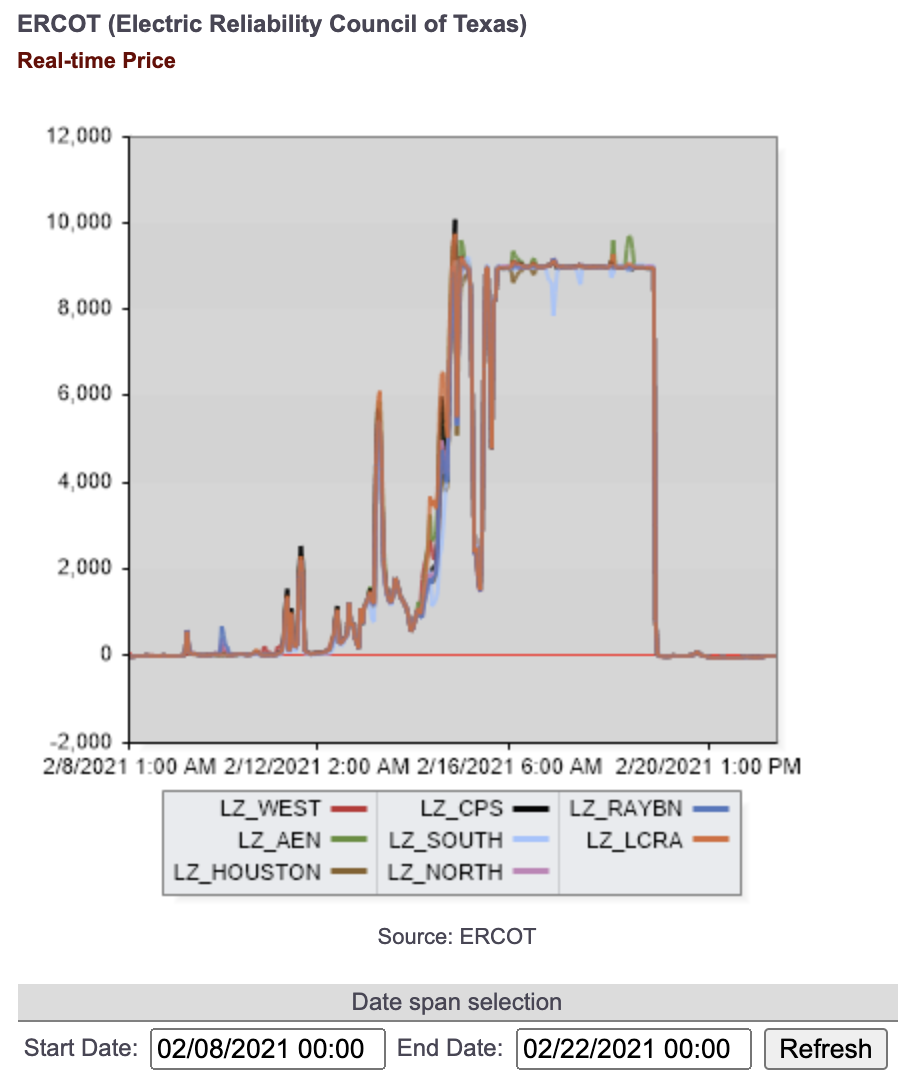
\includegraphics[width=0.65\textwidth]{RTM.png}
\caption{\href{http://www.energyonline.com/Data/GenericData.aspx?DataId=4}{ERCOT Real Time Prices from Feb. 08, 2021 - Feb. 22, 2021}}
\end{figure}
\clearpage
\begin{figure}[h!]
\centering
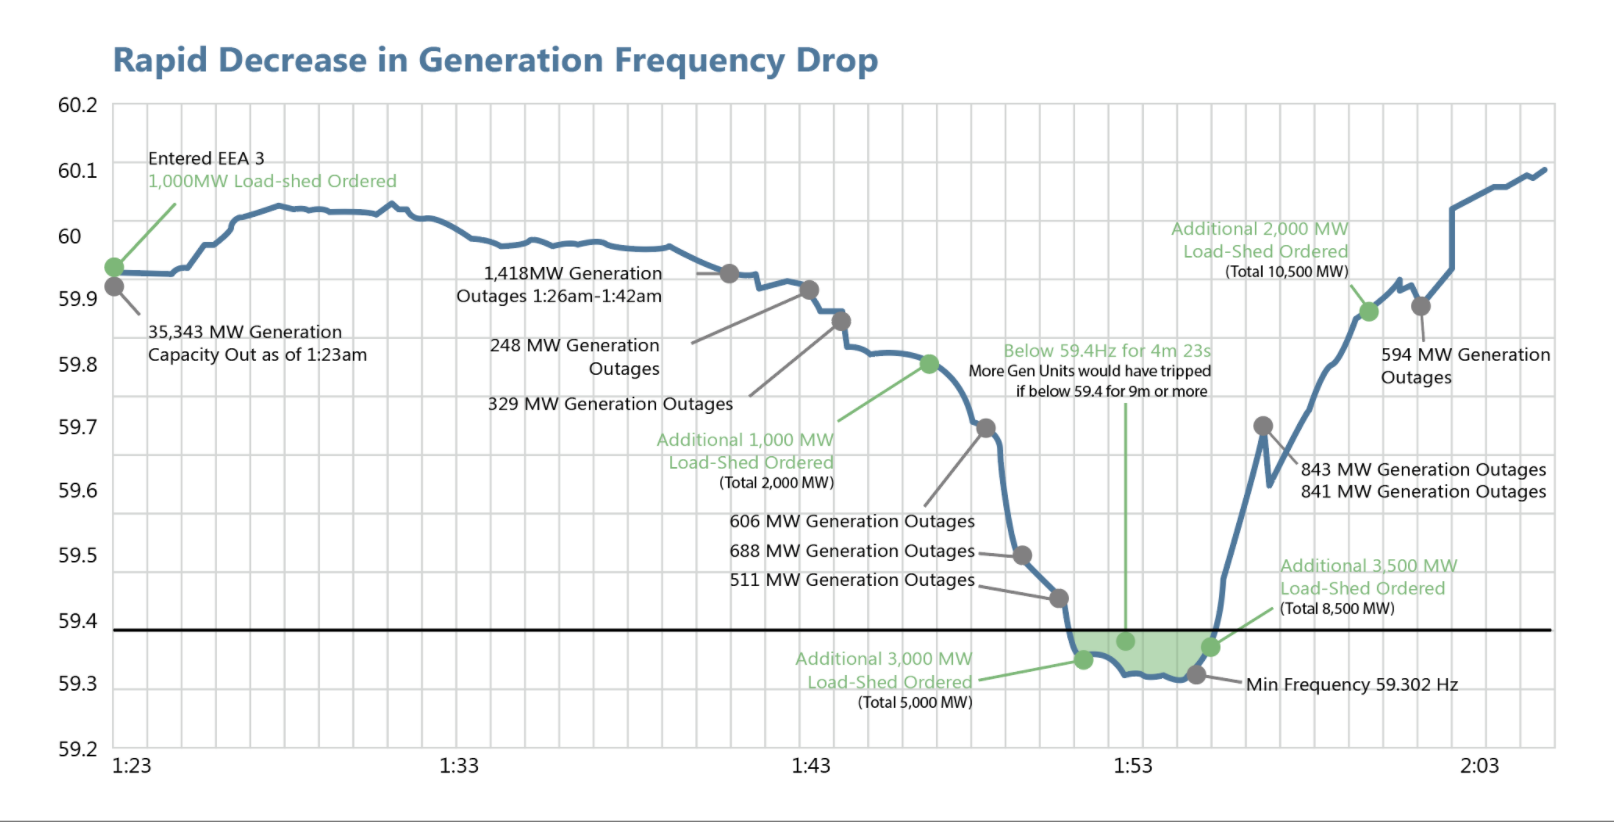
\includegraphics[width=0.85\textwidth]{Screen Shot 2021-04-28 at 4.19.44 PM.png}
\caption{\href{https://powertechresearch.com/texas-power-grid-failure-timeline-of-events-possible-grid-changes-ahead/}{ERCOT Real Time Frequency versus Time on Feb. 15, 2021}}
\end{figure}
%low reserves, bad periodic blackouts to rotate some power to different neighborhoods so everyone would have power periodically rather than some have power all day while others do not for two weeks. 


\section{Discussion: How Can ERCOT Prevent Future Events?}
\indent 
\indent After the smoke cleared there were many topics of conversation that addressed what needs to be fixed in the Texan power grid to prevent future disasters like the one in February 2021 from happening again. The energy-only market in which ERCOT operates has been criticized for not operating as a capacity market, but realistically what a capacity market would do is add to the cost that the consumers would pay and add unreliability to the delivery of that power that was supposedly secured and allocated for the purchaser. Some more realistic approaches that can be considered are the addition of smart meters, temporary insulation of pipelines, uniting ERCOT with neighboring grids, guaranteeing the most significant energy sources that contribute to generation and increasing reserves. I will go over each of these potential improvements and how they would impact the power grid and the market as well. 
\subsection{Adding Smart Meters to Households}
\indent
\indent Smart meters have been becoming increasingly popular throughout the last decade in the United States and are proven to be efficient and cost-friendly mechanisms which play a vital role in the "Smart-grid". These meters allow the distributors to manage the power consumption of every individual household. If bought in bulk quantity, the smart meters may be negotiable at $\$100$ or less per meter, which is great for affordability for the Texan residents. According to studies conducted in 2016 by EIA, Texas has smart meters installed on somewhere in the range of 61\% to 80\% of homes with 2016 accounting for 200,000 installations alone \cite{smartMeterdata}. According to the 2019 Census there are approximately 11.28 million housing units in Texas, so if there are 61\% to 80\% of homes smart metered already, that leaves about 2.25 to 9 million homes that need to get smart metered. If we say each meter will cost $\$100$ then this means to get the remaining homes metered will cost in the range 225 to 900 million dollars. Compared to the damage which has been inflicted from the winter storm (nearly 200 billion in overall damages!) this would be a valuable investment for several reasons. Smart meters give consumers the ability to track their electrical expenditure and keep in mind ways in which to utilize their electricity more efficiently. The smart meters also allow all home owners a fair chance at having sufficient electricity during a load shed event. To put this in perspective, the rotating blackouts which were happening in February 2021 left many homes without power because the load shed events were inefficient. The inefficiency came from the inability to equally distribute the power to all homes in a proper manner and, for example, give neighborhoods A and C power for n number of minutes and then neighborhoods B and D power for n number of minutes. The installation of smart meters are not only beneficial to the power grid to prevent drops in frequency, load shed events and skyrocketing scarcity prices, but this will impact society for the best and prevent deaths that we see were caused by lack of electricity from inefficient rotating blackouts to keep homes warm. 
\subsection{Temporary Pipeline Insulation}
\indent
\indent There has been ongoing debate on whether or not the Texan power grid needs to be weatherized to accommodate for these extreme cold events. To protect against the cold there are two common and logical proposals: bury the pipelines and insulate the pipelines. Spending millions of dollars to insulate the pipelines and generators would be great in a climate that is always cold, but this is not the case in Texas. The heat in Texas would cause the pipes to get dangerously hot and cause more harm than good. The work around to this is to have a temporary insulating protocol for the cold weather anomalies that occur once in a while. A professor from the University of Texas in Austin named Michael Webber noted that weatherization should be temporary to overcome the dichotomy of  overheating a system from permanent insulation and not having enough insulation so that the generators and pipelines risk freezing \cite{mikeWeb}. Not only might this be a favorable and well priced workaround for ERCOT, but it will also offer some more security from a distribution failure for the consumers of energy. If we take a look at the missing sources of generation from Figure 6 we see natural gas was the number one and most critical source which was lost from the very beginning of the outage so finding a workaround to keep this energy source active is critical for the future. By adding a policy which mitigates the losses of natural gas transfer to generators by mandating temporary insulation of pipelines in anticipation of a winter storm, real-time market prices and day-ahead market prices will be more favorable for the market participants and consumers. Being able to provide this kind of distribution security and integrity boosts the reliability and competitiveness of ERCOTs electric market. Although this is not a permanent solution, it is one which may potentially prevent another sequence of power outages across Texas and losses of life. 
\subsection{Uniting ERCOT with Neighboring Grid(s)}
\indent
\indent Uniting ERCOT with neighboring grids has many advantages as noted in this interview of Peter Fairley \cite{wdushtg}. If the grid which ERCOT operates were to unite with neighboring grids it would have additional sources that it would be able to draw power from and use as back up in vital circumstances when demand is not able to be met under unanticipated events or if a generator goes down. This is what improves the reliability of a grid and improves odds of neighborhoods not having days-long blackouts. Utilizing DC interconnections to unite the ERCOT grid with neighboring grids is a great idea because DC is known to have less losses and more efficient transmission of current. Financially there is also an incentive to uniting ERCOT with neighboring grids because while one half of the grid is offline, the other half of the grid may be generating electricity and allocating some of that generated electricity to reserves and transmitted eastward or westward \cite{wdushtg}. This means that the grids can meet demand more efficiently, reliably and the incentive is greater. Of course geographically there is a challenge because there is a physical barrier that makes uniting the Texan grid with neighbors challenging but getting past this obstacle will improve the social welfare as well as increase reliability. A merger could also benefit ERCOT because they may be able to operate as an energy only market and without the need to converge towards a capacity market or in between. 
\subsection{Choice of Energy Sources}
\indent 
\indent Another point of failure from the February 2021 power outages came from the choice of energy sources. As mentioned before, Texas' energy use is approximately 46\% natural gas and 23\% wind according to Figure 1. If we take a look at Figure 6 we can see which energy sources were out of generation and accounting for missing capacity. The majority was coming from natural gas and wind renewables. 

\begin{figure}[h!]
\centering
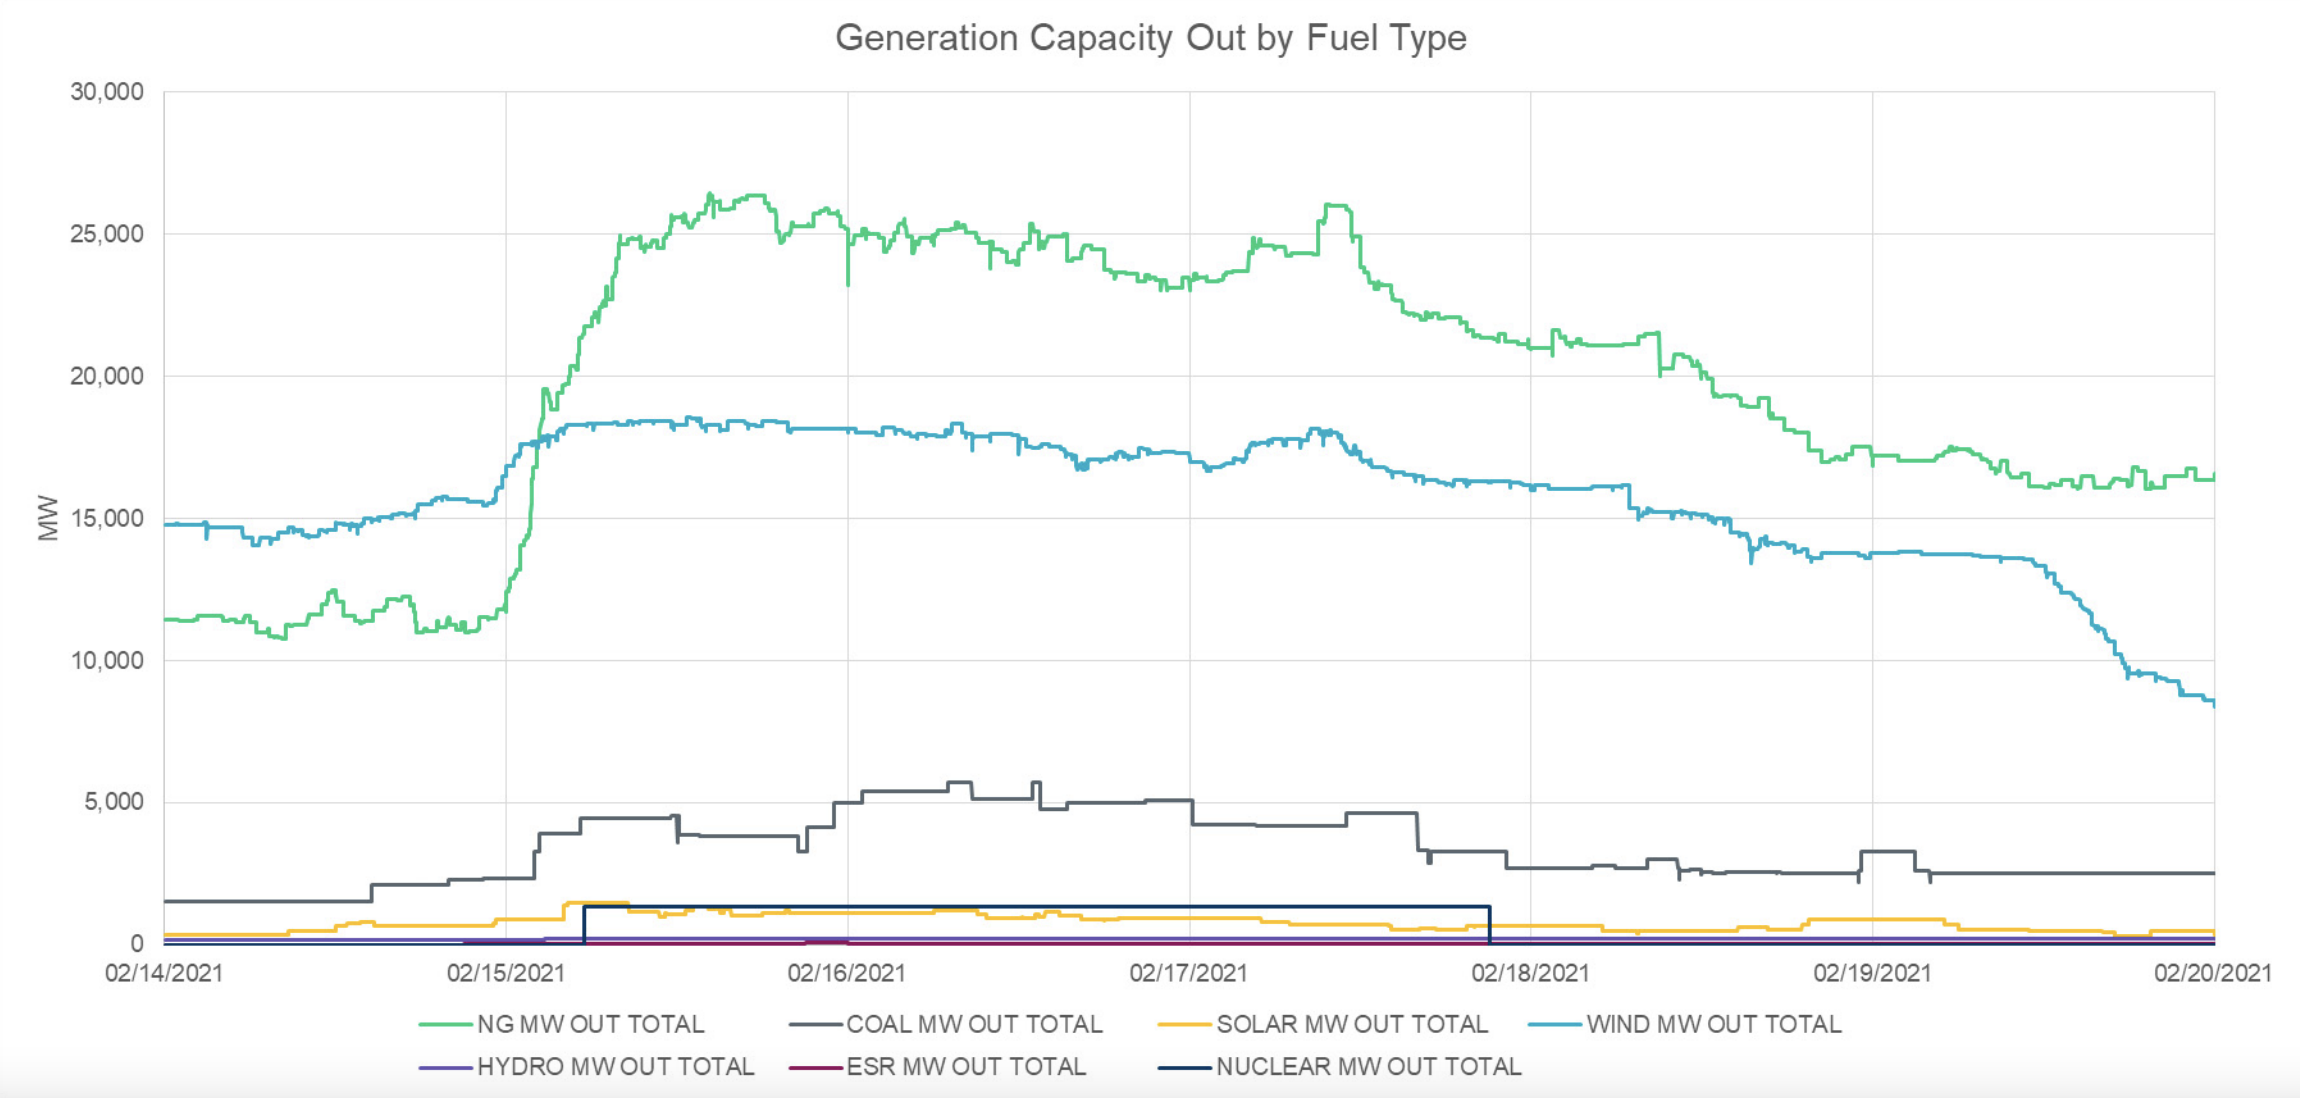
\includegraphics[width=0.65\textwidth]{Screen Shot 2021-04-29 at 10.06.23 AM.png}
\caption{\href{http://www.ercot.com/content/wcm/lists/226271/Texas_Legislature_Hearings_2-25-2021.pdf}{Generation Capacity Out During February 2021 Outage}}
\end{figure}

\noindent From Figure 6 we can deduce where the problems stemmed from and is a great starting point to figure out what can be done to mitigate distribution failures to generators and bring in generation from reserves or a neighboring grid. Solutions to this problem can be as simple as taking care of the distribution aspect so that there aren't discontinuities in the transmission of natural gas to power the generators. There is also another possible solution as well, which would be to diversify the portfolio of the energy sources used during the storm. The sources which would be used could be more coal and maybe even some pumped hydro in the future. South-east Texas should take advantage of being by the ocean and incentivise pumped hydro to generate electricity. However, by far the most reliable long term solution downed generators would be having guaranteed reserves from neighboring grids as mentioned before. The increase of reliability would increase social welfare monumentally and save lives during another catastrophic power outage event. 

\subsection{Increasing Reserves for Additional Demand Security}
\indent
\indent ERCOT currently plans to implement a policy which increases the reserve margin from 2021 through 2025 \cite{ERCOT202-5incReserves}. According to Figure 7 the reserve margins are calculated with the following equation: Reserve Margin as Percent  = $\frac{\lvert MW Planned - MW Currently Installed \rvert}{MW Currently Installed}*100$

\indent There are some very good reasons for needing to increase the reserve margin which ERCOT operates. Having low reserve margins means that there is little generation that is left over after the predicted demand has been met. This reserve margin is what is tucked away for unexpected events such as downed generators or unexpected spikes in demand that need to be met to keep the grid in sync. When the reserve margin is large that is because there is more generation left over after meeting the theoretical peak load and again, is stored away for unexpected circumstances. \par
\indent By this note, ERCOT is doing the right thing by maintaining larger reserve margin for forecasted peak demand. These increases in reserve margins will not only help prevent capacity related power shortages but it will more efficiently allow ERCOT to rotate blackouts if the power grid is unable to meet demands. If we take a look at Figure 8 we get a good idea where ERCOT is going with increasing the reserve margins. It is clear that the frequency of failure events are decreasing as reserve margins increase. This is because more reserve capacity means fewer long-term inability to meet demand events, fewer long-term deviations in frequency and thus a more reliable system. If there is a slimmer reserve margin then scarcity pricing goes up as per the Operating Demand Reserve Curve. 

\begin{figure}[h!]
\centering
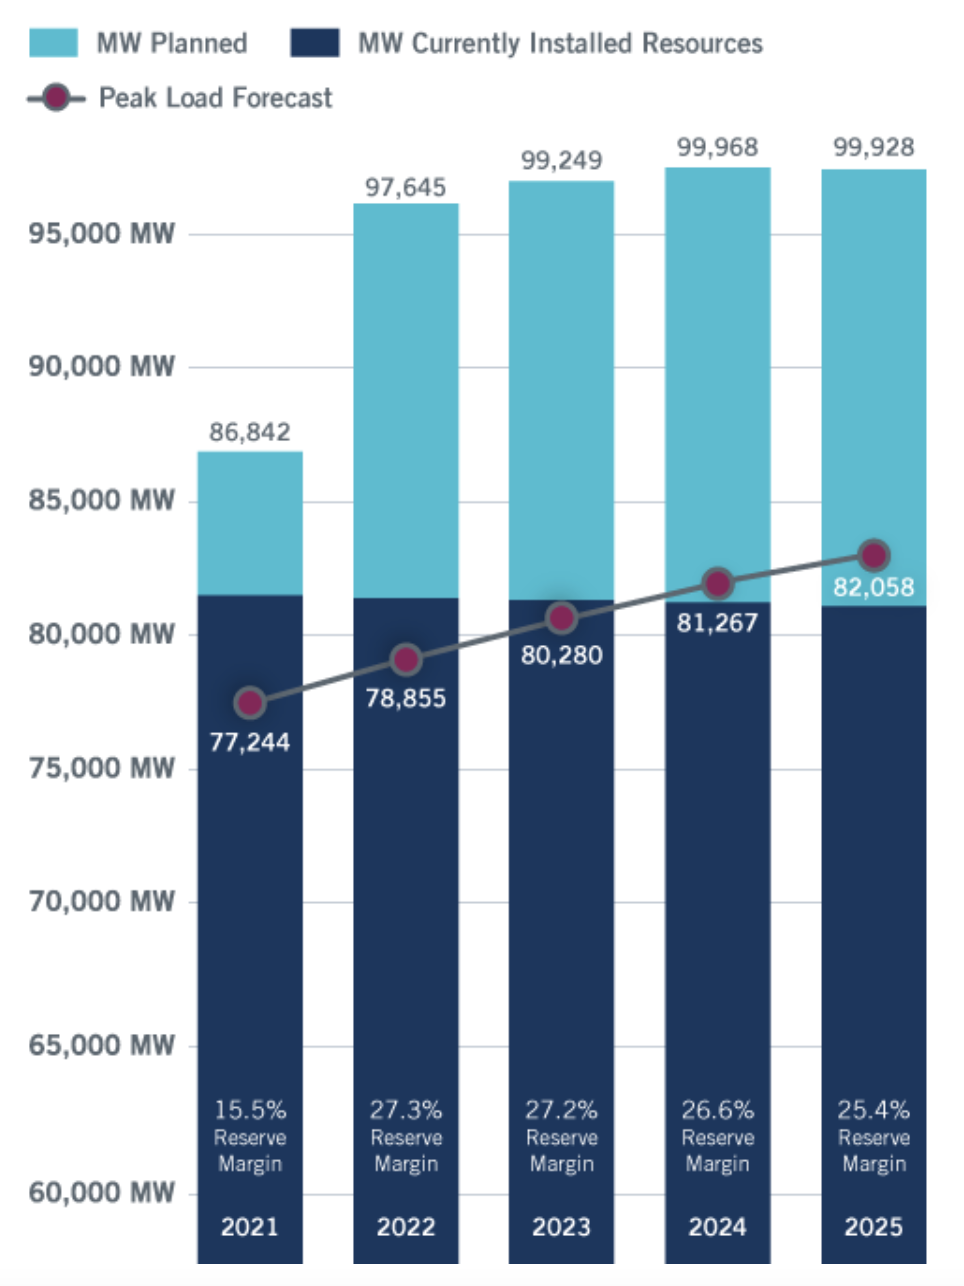
\includegraphics[width=0.45\textwidth]{Screen Shot 2021-04-28 at 11.44.43 PM.png}
\caption{\href{http://www.ercot.com/news/releases/show/219347#:~:text=AUSTIN}{ERCOT Future Reserve Margins Proposed 2020}}
\end{figure}

\begin{figure}[h!]
\centering
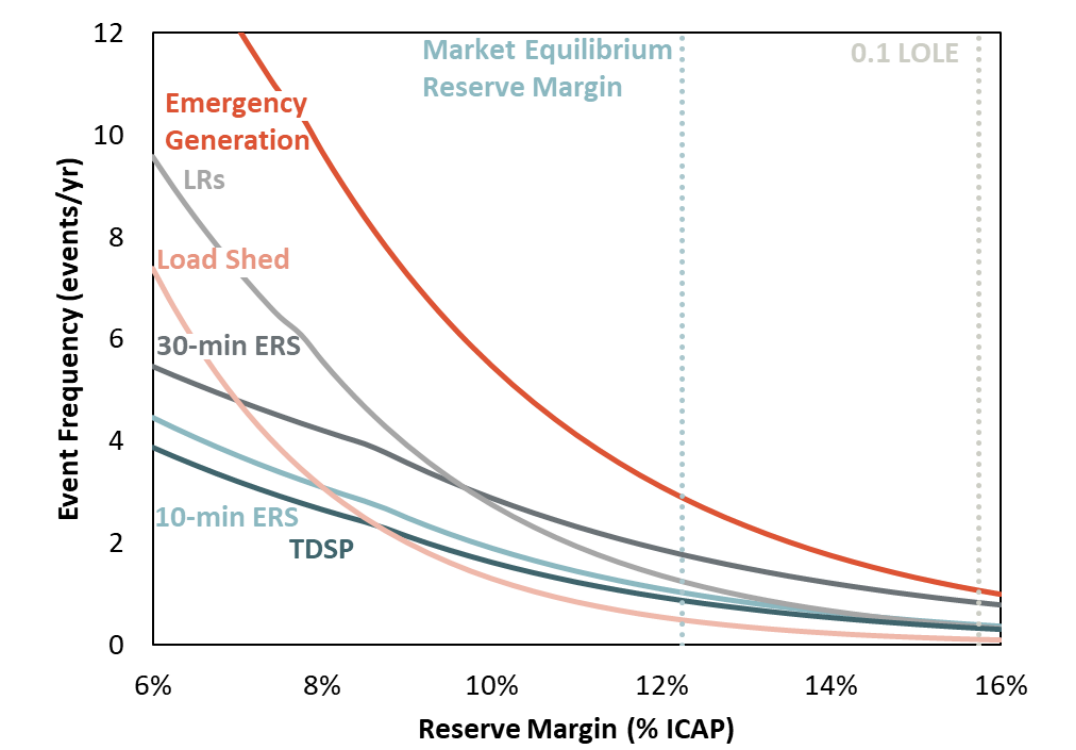
\includegraphics[width=0.65\textwidth]{Screen Shot 2021-04-29 at 8.07.23 AM.png}
\caption{\href{http://www.ercot.com/content/wcm/lists/219844/2020_ERCOT_Reserve_Margin_Study_Report_FINAL_1-15-2021.pdf}{Average Annual Number Failure Events vs Reserve Margin}}
\end{figure}
\clearpage

\section{Conclusion}
\indent
\indent The most beneficial, realistic and achievable moves for ERCOT towards improving the reliability of their grid and modernizing their grid would be 1) making their energy sources more reliable under unpredictable weather, 2) unite with a neighboring grid(s) so that they are not entirely operating on their own and 3) installing smart meters to the remaining homes to help mitigate demand and rotate blackouts more effectively. If ERCOT unites with a neighboring grid or grids this does not mean they need to always tap into their power and participate in their market, but when there is dire need for power like in the case of the February outages it would be wise to mingle in another market to meet the demands and buy ERCOT more time to devise a strategy which would bring the network back up to speed. Broadening the energy types which contribute to generation in ERCOTs market would not help in another snow storm with freezing temperatures because it would cause the capacities of the current generators to be driven at full capacity which would impact the life of the generator. Instead of changing the energy source portfolio, what would improve the reliability of the system incredibly is the temporary insulation of the gas pipelines and generators in anticipation of the storms, that way there is a larger probability in meeting the majority of demand and not dealing with frozen pipelines and downed generators. In addition, modernization of the grid and developing a smarter network  with interconnected feeders which would strategically supply neighborhoods which would otherwise have been left powerless in a crisis. Although uniting grids is not in ERCOTs plans yet it would pay off in the long term by providing reliability and financial gain. This strategy would make optimal scheduling more efficient so they don't need to worry so much about not meeting demand since they would have back up from their neighbors, if needed.\par
\indent The 20\% contribution from wind energy to the energy capacity of the market is another worrisome topic which resulted after the outages were fixed. In the case of the cold winter storm, wind generation was completely out of the generation market and this left question marks on whether wind renewables are the most optimal renewable that is can help support ERCOT and its market. The real question here is how can wind renewables be made more efficient to participate in the energy market. Some ways which might mitigate the propellers freezing over could be to use ethylene- or propylene-glycol to deice them, just as it is utilized on the airfoils of an aircraft. Utilising the concepts of antifreeze coolant as in automobiles may also be efficient in warming the propellers to not ice over. It is still early in the development of renewable energy sources and many of them can be improved to help in the energy market under a broad set of circumstances. \par
\indent After our discussion on the effects of removing capacity from the market on scarcity prices and the Operating Demand Reserve Curve we can conclude that the market is operating in a way that benefits the stakeholders of the capacity market. The reason is because there is an intentional design to keep prices high during low reserves in order to bring generation back up to capacity when generators are out and not meeting demand. The most significant workarounds that should be looked at are those for installing smart meters to the remainder of homes in Texas, temporarily insulating pipelines in advance of the storms and figuring out how to make renewables work under the complex winter storm environmental factors so that they participate in the market at all times.

\begin{figure}[h!]
\centering
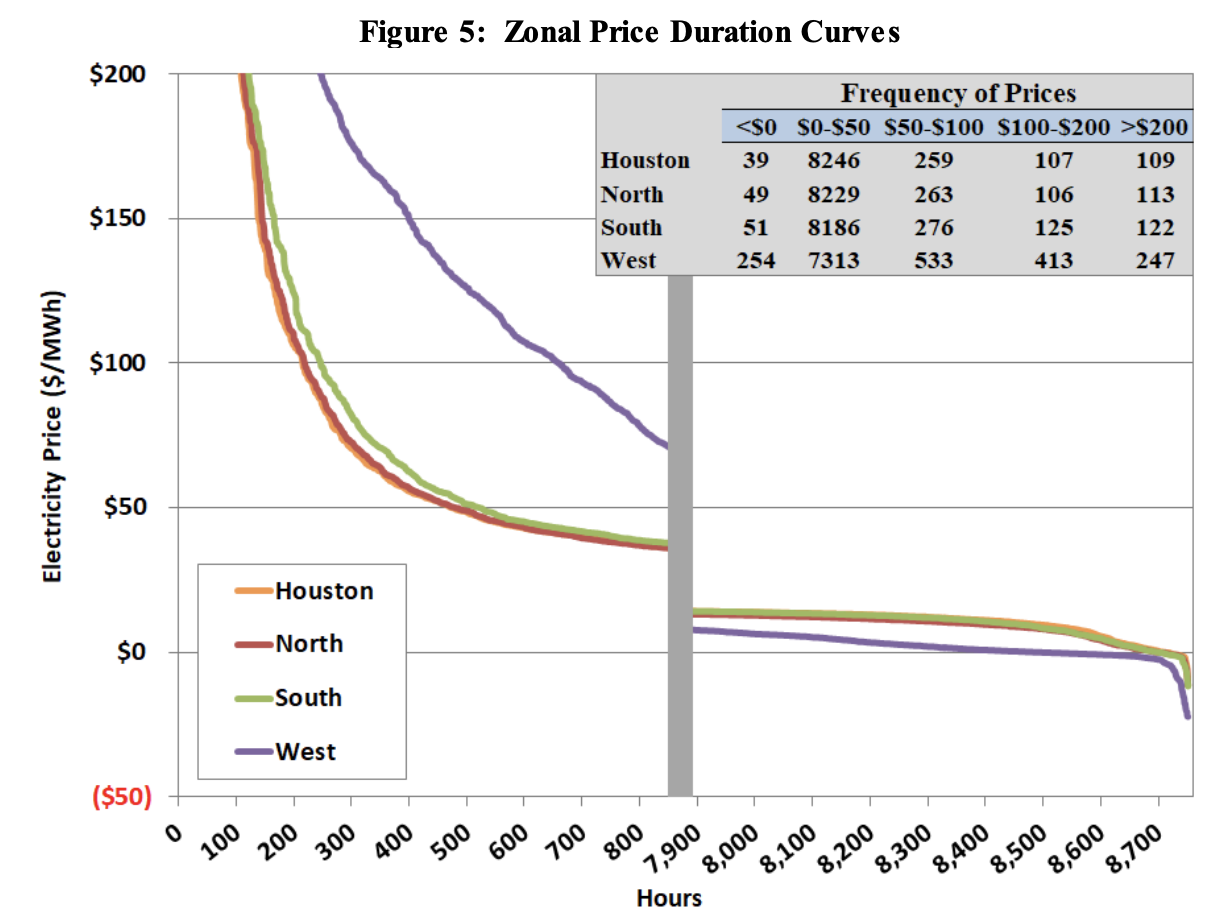
\includegraphics[width=0.65\textwidth]{Screen Shot 2021-04-28 at 4.58.48 PM.png}
\caption{\href{https://rtoinsider.com/wp-content/uploads/2019-State-of-the-Market-Report.pdf}{ERCOT Price Duration Curve 2019 of Top and Bottom 10\%}}
\end{figure}

\clearpage
\section{Acknowledgements}
\indent
\indent I want to thank Professor Caramanis, who taught the EC 543 course at Boston University, for his diligence and thorough recommendations for topics to write about for this report. I also want to thank those authors, writers and sites from where I pulled information from and cited in my references. Transmission and distribution networks are never talked about in the real-world and creating this paper has been a journey, proving this field of work involves not only sophisticated engineering but careful marketing as well. \par 
\indent All references are at the end of sentences and paragraphs with corresponding hyperlinks that will take you to the exact reference, which also has a hyperlink to the online sites where I was able to find the information needed. All figures used in this report also have hyperlinks under them in the caption which can take you to the source where the data was found. 
\cleardoublepage
\phantomsection
\addcontentsline{toc}{section}{References}
\printbibliography{}


\end{document}